\documentclass[twoside]{article}

\usepackage[math]{kurier}
\usepackage[sc]{mathpazo}
\renewcommand{\sfdefault}{kurier}

\usepackage{amsmath}
\usepackage{amssymb}
\usepackage{graphicx}
\setlength{\oddsidemargin}{0.25 in}
\setlength{\evensidemargin}{-0.25 in}
\setlength{\topmargin}{-0.6 in}
\setlength{\textwidth}{6.5 in}
\setlength{\textheight}{8.5 in}
\setlength{\headsep}{0.75 in}
\setlength{\parindent}{0 in}
\setlength{\parskip}{0.1 in}


\newcounter{lecnum}
\renewcommand{\thepage}{\thelecnum-\arabic{page}}
\renewcommand{\thesection}{\thelecnum.\arabic{section}}
\renewcommand{\theequation}{\thelecnum.\arabic{equation}}
\renewcommand{\thefigure}{\thelecnum.\arabic{figure}}
\renewcommand{\thetable}{\thelecnum.\arabic{table}}


\newcommand{\lecture}[3]{
   \pagestyle{myheadings}
   \thispagestyle{plain}
   \newpage
   \setcounter{lecnum}{#1}
   \setcounter{page}{1}
   \noindent
   \begin{center}
   \framebox{
      \vbox{\vspace{2mm}
    \hbox to 6.28in { {\bf \sffamily AA 274: Principles of Robotic Autonomy
                        \hfill Winter 2018} }
       \vspace{4mm}
       \hbox to 6.28in { {\sffamily{\Large \hfill Lecture #1: #2  \hfill}} }
       \vspace{2mm}
       % \hbox to 6.28in { {\it \hfill Scribes: #4} }
      \vspace{2mm}}
   }
   \end{center}
   \markboth{Lecture #1: #2}{Lecture #1: #2}

   \vspace*{4mm}
}



%%%%%%%%%%%%%%%%%%%%%%%%%%
%document
\begin{document}
%modify this
\lecture{7}{Image Processing, Feature Detection and Description}{}

\section{Introduction}
This lecture discusses several techniques used to extract information from images. The objective is to learn how to represent images and infer visual content from them by focusing on the three key steps of the image processing pipeline: filtering images, feature detection, and feature description.

While images are represented as a collection of pixel values, this raw data is not very useful to computers without image processing and feature detection.  Our aim is to detect local features, such as corners and edges, in order to identify similarities between images, identify 3D objects, and track objects between frames.

\section{Image Filtering}
We start by considering an image as a function $I$: $[a,b]\times[c,d] \rightarrow [0,L]$, where $I(x,y)$ represents the grayscale pixel intensity at $(x,y)$. Assuming we have a two-dimensional grayscale image, the image is represented as a two-dimensional matrix with $r$ rows and $c$ columns. Each entry is equal to the discretized brightness level; often we use 256 levels, where 0 corresponds to black and 255 to white. For a color image, each entry in the matrix would be a vector function with three components, one each for the red, green, and blue color channels.

Image filtering is the process of accepting and rejecting certain frequency components. Image filters can be implemented in one of two ways: in the frequency domain or in the spatial domain. In this class we will mostly focus on filters in the spatial domain.

\subsection{Spatial Filters}
A spatial filter consists of:
\begin{enumerate}
  \item A neighborhood $S_{xy}$ of pixels around the point $(x,y)$ under examination
  \item A predefined operation $F$ that is performed on the image pixels within $S_{xy}$
\end{enumerate}

Spatial filters can be linear or non-linear. In this class, we will focus on linear spatial filters, given by the equation \ref{linear} below.
\begin{equation}
  \label{linear}
  \begin{aligned}
  	I'(x,y) = F \circ I = \sum_{i=-n}^n \sum_{j=-m}^m F(i,j)I(x+i,y+j)\\
  \end{aligned}
\end{equation}

In equation \ref{linear}, $I'$ represents the filtered image, $F$ represents the filter mask (sometimes called the kernel or window), and $I$ represents the original image. The filter mask $F$ is of size $(2N + 1)\times(2M + 1)$), where each entry represents the weighting of a particular neighbor pixel from the original image.

We apply this filter mask to every pixel $(x,y)$ by multiplying each value of intensity in the neighborhood of $(x,y)$ by a certain weight $F(i,j)$ in order to get to the filtered image $I'$. This procedure is referred to as a \textit{correlation} with the kernel $F$.

\subsubsection{Moving Average}
As an example of a linear spatial filter, the moving average filter returns the average of the pixels in the mask. It achieves a smoothing effect by removing sharp features. For example, for a \textit{normalized} $3\times3$ mask,
\[
F = \frac{1}{9}
\begin{bmatrix}
1 & 1 & 1\\
1 & 1 & 1\\
1 & 1 & 1
\end{bmatrix}
\]
This filter is commonly used to reduce noise and smooth/blur an image, as seen in figure 7.1.

\begin{figure}[h]
	\centering
	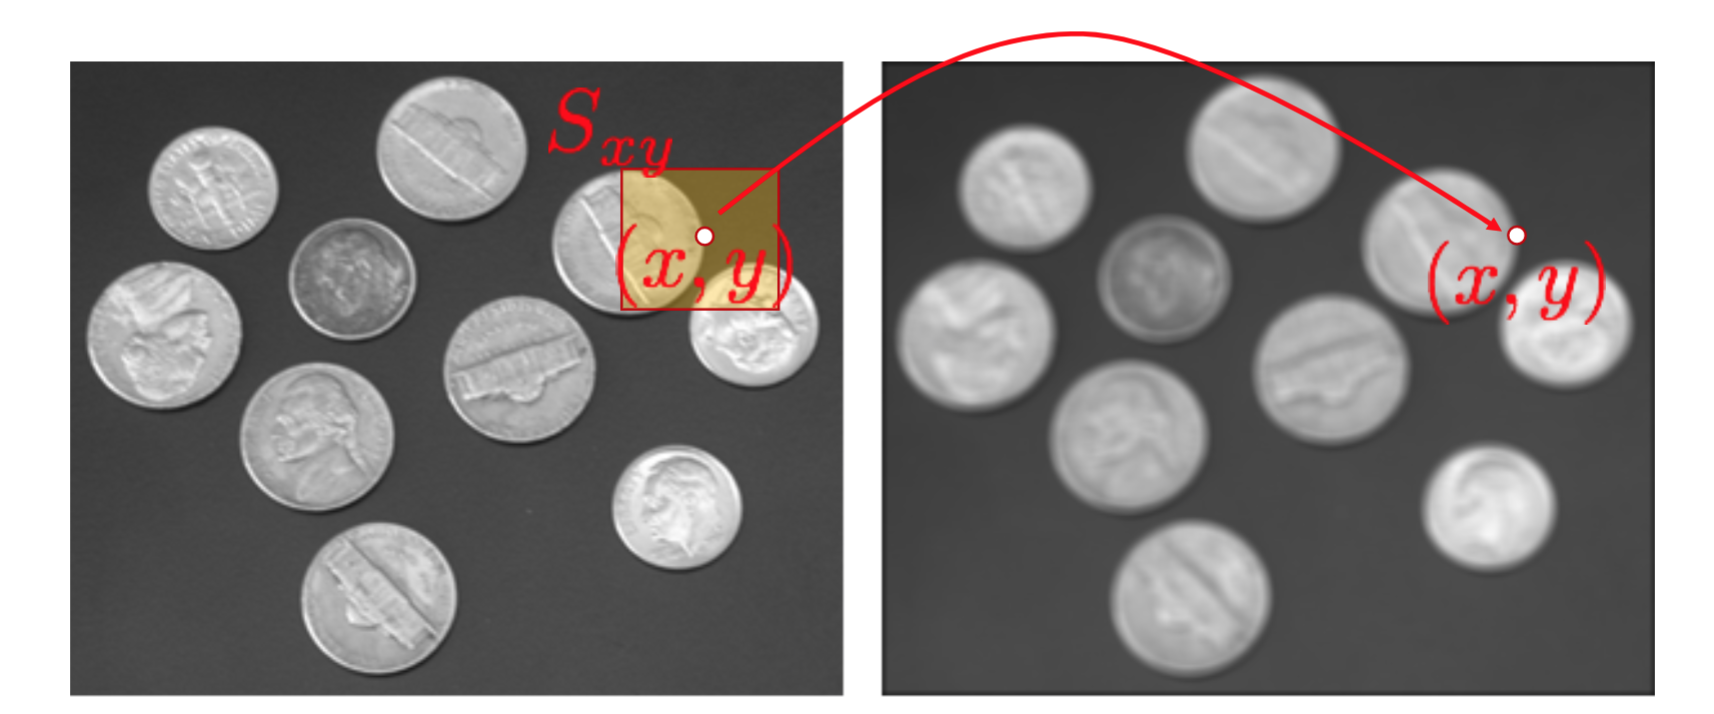
\includegraphics[scale=.4]{blur.png}
    \caption{Example of a moving average filter}
    \label{noisy}
\end{figure}

\subsubsection{Gaussian Smoothing}
Another linear spatial filter, the Gaussian filter, is often preferred over a simple moving average filter because the Gaussian filter gives higher weights to pixels closer to the center of the filter and lower weights to those pixels along the edge. The Gaussian smoothing function is given in equation \ref{gaussian} below.
\begin{equation}
  \label{gaussian}
  \begin{aligned}
  	G_\sigma(x,y) = \frac{1}{2\pi\sigma^2} \exp \bigg(-\frac{x^2 + y^2}{2\sigma^2} \bigg)\\
  \end{aligned}
\end{equation}
The function is sampled about its center to obtain the mask. For example, for a normalized $3\times3$ mask with $\sigma$ = 0.85,
\[
G = \frac{1}{16}
\begin{bmatrix}
1 & 2 & 1\\
2 & 4 & 2\\
1 & 2 & 1
\end{bmatrix}
\]

\subsubsection{Convolution}
Convolution is a linear filter that is similar to correlation, but has reverse image indices. Correlation and convolution are identical when the filter is symmetric. The convolution equation is shown in \ref{convolution}.

\begin{equation}
  \label{convolution}
  \begin{aligned}
  	I'(x,y) = F * I = \sum_{i=-n}^n \sum_{j=-m}^m F(i,j)I(x-i,y-j)\\
  \end{aligned}
\end{equation}

Convolution enjoys the associativity property $F*(G*I) = (F*G)*I$. We commonly use this associativity property when smoothing an image and taking the derivative of the resulting image.  We can combine these two operations into one by first convolving the derivative filter with the Gaussian filter, then convolving the resulting filter with the image.  This second approach is advantageous because it is less computationally intensive.

\subsubsection{Separable Masks}
A mask is separable if it can be broken down into the convolution of two kernels $F = F_1 * F_2$. If a mask is separable into ``smaller'' masks, then it is often cheaper to apply $F_1$ followed by $F_2$, rather than by $F$ directly. There is a special case where the mask is representable as outer product of two vectors (equivalent to two-dimensional convolution of those two vectors). If the mask is $M\times M$, and the image has size $w\times h$, then the complexity is $O(M^2wh)$ with no separability or $O(2Mwh)$ with separability into the outer product of two vectors.

The moving average mask can be separated as shown below.
\[
F = \frac{1}{9}
\begin{bmatrix}
1 & 1 & 1\\
1 & 1 & 1\\
1 & 1 & 1
\end{bmatrix} = \frac{1}{9}
\begin{bmatrix}
1 \\
1 \\
1
\end{bmatrix}
\begin{bmatrix}
1 & 1 & 1\\
\end{bmatrix}
\]

The Gaussian mask is also separable because the exponential function can be separated out. The Gaussian smoothing separable mask is shown below in equation \ref{gausmask}.
\begin{equation}
\label{gausmask}
  \begin{aligned}
  	G_\sigma(x,y) = \frac{1}{2\pi\sigma^2} \exp \bigg(-\frac{x^2 + y^2}{2\sigma^2} \bigg)\\
    = \frac{1}{\sqrt{2\pi}\sigma}\exp \bigg(-\frac{x^2}{2\sigma^2}\bigg)\frac{1}{\sqrt{2\pi}\sigma} \exp \bigg(-\frac{y^2}{2\sigma^2}\bigg) \\
    = g_\sigma(x) \cdot g_\sigma(y)
  \end{aligned}
\end{equation}

Decomposing a mask into its separable components does not alter the results but can drastically affect the computational speed of your code.

\section{Image Differentiation}
Taking the derivative of an image is similar to differentiating a function with a two-dimensional domain. On a basic level, the derivative of an image represents changes in pixel intensity in both the vertical and horizontal direction. Because images are discrete functions, the traditional method for differentiating continuous functions can not be used. One popular method to differentiate an image is known as the central difference method; the equations for this method are shown below in equation \ref{cendiff}. These equations find the change in intensity between the neighboring pixels.

\begin{equation}
  \label{cendiff}
  \begin{aligned}
    \frac{\partial I} {\partial x} &= I(x+1,y) - I(x-1,y)\\
    \frac{\partial I} {\partial y} &= I(x,y+1) - I(x,y-1)
  \end{aligned}
\end{equation}

Here, $I$ is the intensity of the image, and $x$ and $y$ define the location of the pixel of interest. Note that applying a normalization factor to these equations does not effectively change the result, as the background intensities will be scaled by the same factor. The derivative with respect to $x$ is the derivative in the horizontal direction, and the derivative with respect to $y$ is in the vertical direction. The central difference method looks at the neighboring pixels on both sides of the pixel of interest. It is also valid to just consider one side of each pixel to calculate the derivative, for example $\frac{\partial I}{\partial x} = I(x+1,y) - I(x,y)$. While this method would be correct, using both neighboring sides is generally better at estimating the derivative right at the pixel of interest.

It is also possible to differentiate an image using convolution operations, such as with a Sobel mask.  Sobel masks work similarly to the masks discussed earlier in this lecture. The Sobel masks for the $x$ and $y$ direction are given below.

\[
S_x =
\begin{bmatrix}
1 & 0 & -1\\
2 & 0 & -2\\
1 & 0 & -1
\end{bmatrix}
, \qquad S_y =
\begin{bmatrix}
1 & 2 & 1\\
0 & 0 & 0\\
-1 & -2 & -1
\end{bmatrix}
\]

Sobol masks are similar to the central difference method described above in that both approaches use the intensity of neighboring pixels to find the derivative, but Sobol masks use more neighboring pixels when calculating the derivative.

For example, $S_x$ weights the rows above and below the row of interest to calculate the horizontal derivative, and $S_y$ weights the columns above and below the column of interest to find the vertical derivative. In essence, the $S_x$ operator takes the central difference of the the row of interest, as well as the rows above and below below the pixel location, and then takes a weighted average of those central differences to make the differentiation more robust.


\subsection{Similarity Measures}
Filtering can be used to find similar features in different images. Two useful examples of similarity measures are the sum of absolute differences (SAD) and the sum of squared differences (SSD). The equations for each are given below in (\ref{SAD}) and (\ref{SSD}), respectively.

\begin{equation}
  \label{SAD}
  \begin{aligned}
  	SAD = \sum_{i=-n}^n \sum_{j=-m}^m |I_1(x+i,y+j)-I_2(x^\prime+i,y^\prime+j)|\\
  \end{aligned}
\end{equation}
\begin{equation}
  \label{SSD}
  \begin{aligned}
	SSD = \sum_{i=-n}^n \sum_{j=-m}^m [I_1(x+i,y+j)-I_2(x^\prime+i,y^\prime+j)]^2
  \end{aligned}
\end{equation}

In these equations, $x$ and $y$ refer to a point in image $I_1$, and $x^\prime$ and $y^\prime$ refer to a point in image $I_2$.
The width and height of the patch, in pixels, are denoted by $n$ and $m$, respectively. SAD and SSD tend not to be very robust, but they do provide a starting point for comparing image features.


%\section{Detectors (general)}
%The goal of detectors is to detect local features. The lecture 7 slides define features as, “image patterns that differ from the immediate neighborhood in terms of intensity, color, or texture.” Some examples of features are edges, corners, and blobs.

%Identifying corresponding features in different images has limitless applications. Some previously discussed applications which require feature detection include 3-D reconstruction, epipolar geometry, and camera calibration.



\section{Image Feature Extraction}

A local feature on an image can often also be referred to as an interest point, interest region, or keypoint - it is an image pattern where the intensity, color or texture differs from its immediate neighborhood. Often times, such as in medical image processing or automotive applications, local features have semantic interpretations, such as blobs corresponding to blood cells in medical images or edges corresponding to the lane of the road. There are also some features that do not possess semantic content but their locations can be found consistently and robustly overtime, which is valuable for uses such as feature tracking, camera calibration, 3D reconstruction, image mosaicing and panorama stitching. In some cases, the location of the features does not matter either; for applications such as scene classification, texture analysis, video mining, and image retrieval, only the number of feature matches is important. This section discusses the basic concepts of some local feature extractors (detectors and descriptors), and their desired properties.

\subsection{Detectors}
Detectors detect local features. The most common detectors are edge detectors, corner detectors and blob detectors.
\subsubsection{Edge Detection}
\textbf{Introduction}\\
Let us define an edge as ``a region in an image where there is a significant change in intensity values along one direction, and negligible change along the orthogonal direction.'' In one dimension, an edge corresponds to a point where there is a sharp change in intensity, or more explicitly, a large first derivative and a small second derivative. Many edge detectors rely on differentiating images and looking for spikes in the derivative.

Some criteria necessary for robust edge detection include accuracy, localization, and single response. To elaborate, good accuracy implies few false positives or negatives.  Localization refers to the placement of the detected edge - the edge should be exactly where the true edge is, not offset or rotated. Finally, single response means one edge is detected for each real edge. For example, one real edge should not be detected as two separate edges.

Most edge detection methods rely on two key steps, smoothing and differentiation. Differentiation is performed in both the vertical and horizontal directions to find locations with high intensity gradients in just one of the two directions. However, just differentiating an image is vulnerable to issues with noise and random single pixels which may have high intensity gradients. To account for this, many algorithms will smooth the image before differentiating it, eliminating noisy pixels. The next section explores edge detection further. \\

\textbf{Techniques}\\
In this part we will discuss classic edge detection techniques. They involve the use of convolution with a Kernel to extract edges. For example, differentiating every point in our signal should only give non zero values (or at least high values) at each edge, allowing us to sort them easily. However we will see that this is not always the case as our signal/image is usually not as smooth as we would like it to be.

Let us first explore the 1D case to understand the principle of edge detectors and how they behave under high noise. For example, looking at \ref{noisy}, we see that simply differentiating the signal without performing any sort of filtering will yield a completely useless result, as noise causes random values of the derivative at every point. There is no detection threshold that will allow us to detect edges from this differentiated signal.

\begin{figure}[h]
	\centering
	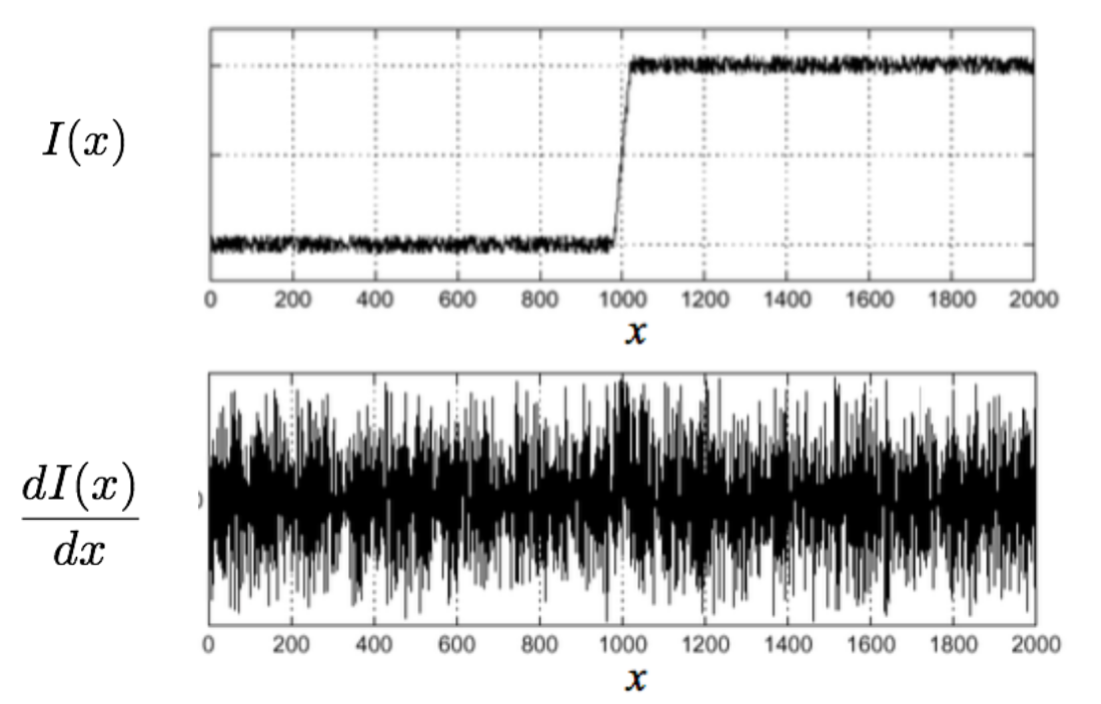
\includegraphics[scale=.4]{noisy_uncorrected.PNG}
    \caption{Differentiation of a noisy signal}
    \label{noisy}
\end{figure}

We can remedy this problem by filtering the signal. For example we may use a Gaussian filter to apply a smoothing mask, the result of which can be differentiated to identify edges (by identifying the highest value or the point where the second derivative cancels). To do so, we perform the following convolutions:
\begin{gather*}
s(x)=g_\sigma(x) * I(x)\\
s'(x)=\frac{d}{dx} * s(x)
\end{gather*}
Where $I$ is the original signal, $g_\sigma$ is the Gaussian, and $s'$ is the final mask. The performance of such a procedure may be seen in \ref{gauss}.

\begin{figure}[h]
	\centering
	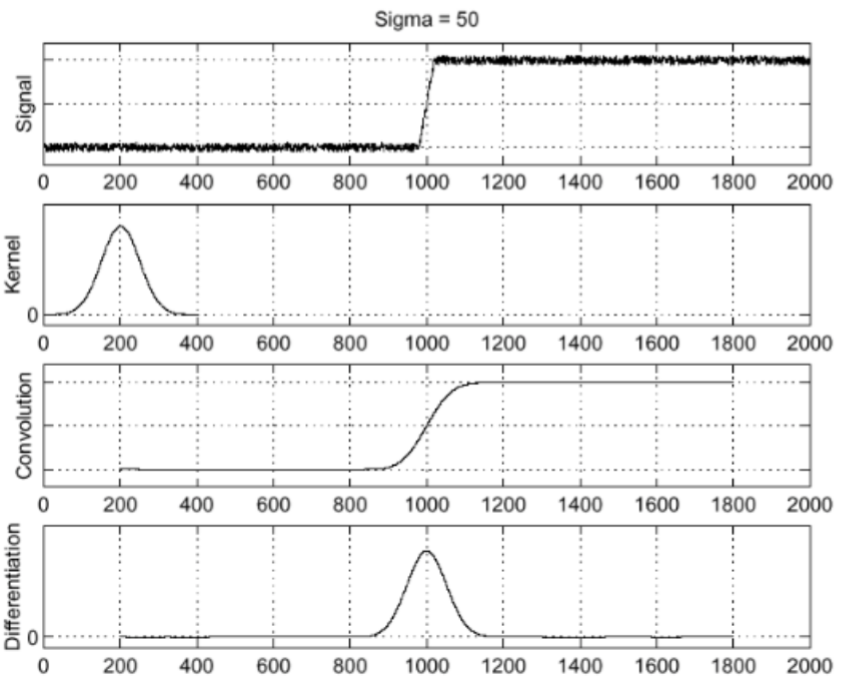
\includegraphics[scale=.4]{gaussian.PNG}
    \caption{Edge detection through convolution with Gaussian kernel, followed by differentiation}
    \label{gauss}
\end{figure}

One issue with this method is that it requires that we compute two convolutions on our image, which can be computationally expensive. It is possible to exploit the associativity of the convolution to perform the same transformation with a single convolution:
\begin{gather*}
s'=\frac{d}{dx} * (g_\sigma * I)=(\frac{d}{dx} * g_\sigma) * I
\end{gather*}
Therefore the function $g'_\sigma=\frac{d}{dx} * g_\sigma$ may be used for much faster computation. An illustration of this process may be seen in \ref{ker}.

\begin{figure}[h]
	\centering
	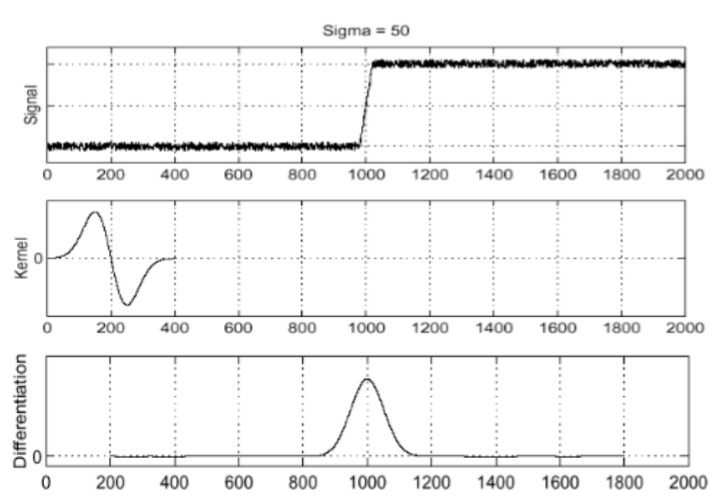
\includegraphics[scale=.5]{better_kernel.PNG}
    \caption{Edge detection through convolution with a differentiated Gaussian kernel}
    \label{ker}
\end{figure}

Now we might take inspiration from this 1D case to design a 2D edge detector. Let $G_\sigma$ be the two dimensional Gaussian distribution (i.e. $G_\sigma(x,y)=\frac{1}{2\pi\sigma^2}exp\bigg(-\frac{x^2+y^2}{2\sigma^2}\bigg)$). An illustration of this function and its derivative may be found in \ref{2dgauss}.

\begin{figure}[h]
	\centering
	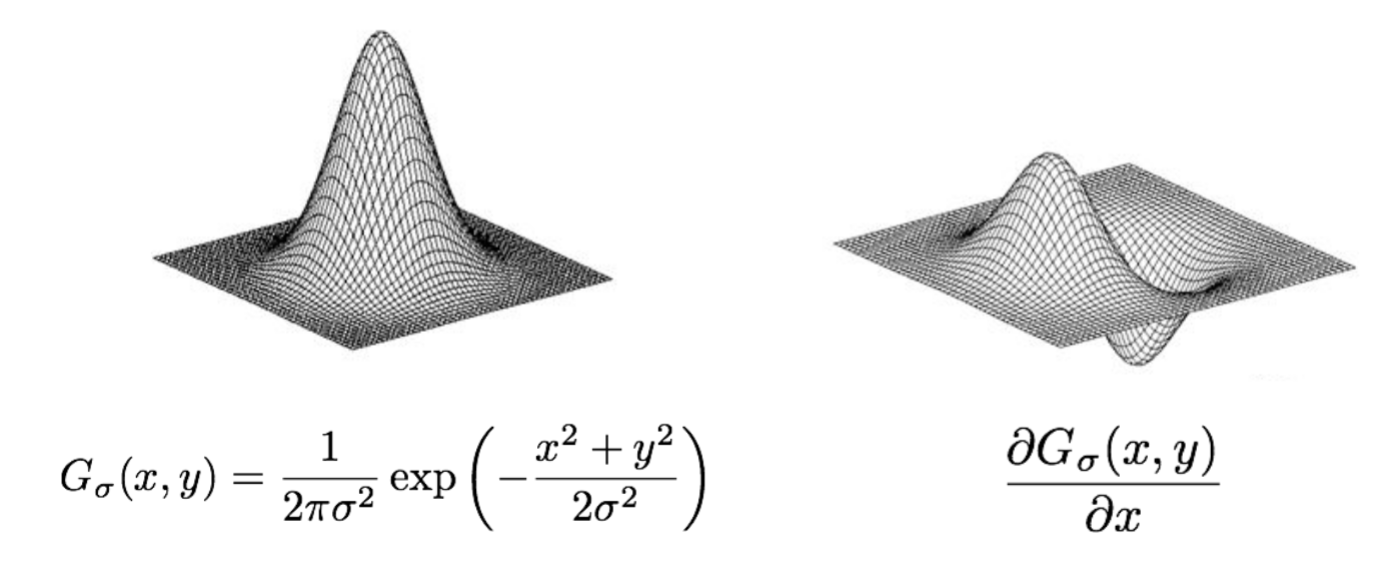
\includegraphics[scale=.3]{2d_equivalent.PNG}
    \caption{2D Gaussian function}
    \label{2dgauss}
\end{figure}

The gradient of the smoothed image may be written as:
\begin{gather*}
\nabla S= \begin{bmatrix}
\frac{\partial}{\partial x} * G_\sigma * I \\ \frac{\partial}{\partial y} * G_\sigma * I \end{bmatrix}= \begin{bmatrix}
G_{\sigma,x} * I\\G_{\sigma,y} * I
\end{bmatrix}=\begin{bmatrix}
S_x\\S_y
\end{bmatrix}
\end{gather*}

We notice that once again we are able to reduce the number of convolutions to 1 by building the partial derivatives of the Gaussian: $G_{\sigma,x}$ and $G_{\sigma,y}$. As in the 1D case, our next step is to check $|\nabla S| =\sqrt{S_x^2+S_y^2}$ against an aptly chosen threshold to detect edges. We may additionally filter out points that are above the threshold but not local maxima to guarantee thin edges.

Finally, an application of this method on a picture classically used to demonstrate image processing techniques may be found in \ref{edge_app}.\\

\subsubsection{Corner Detector}

\begin{figure}[h]
	\centering
	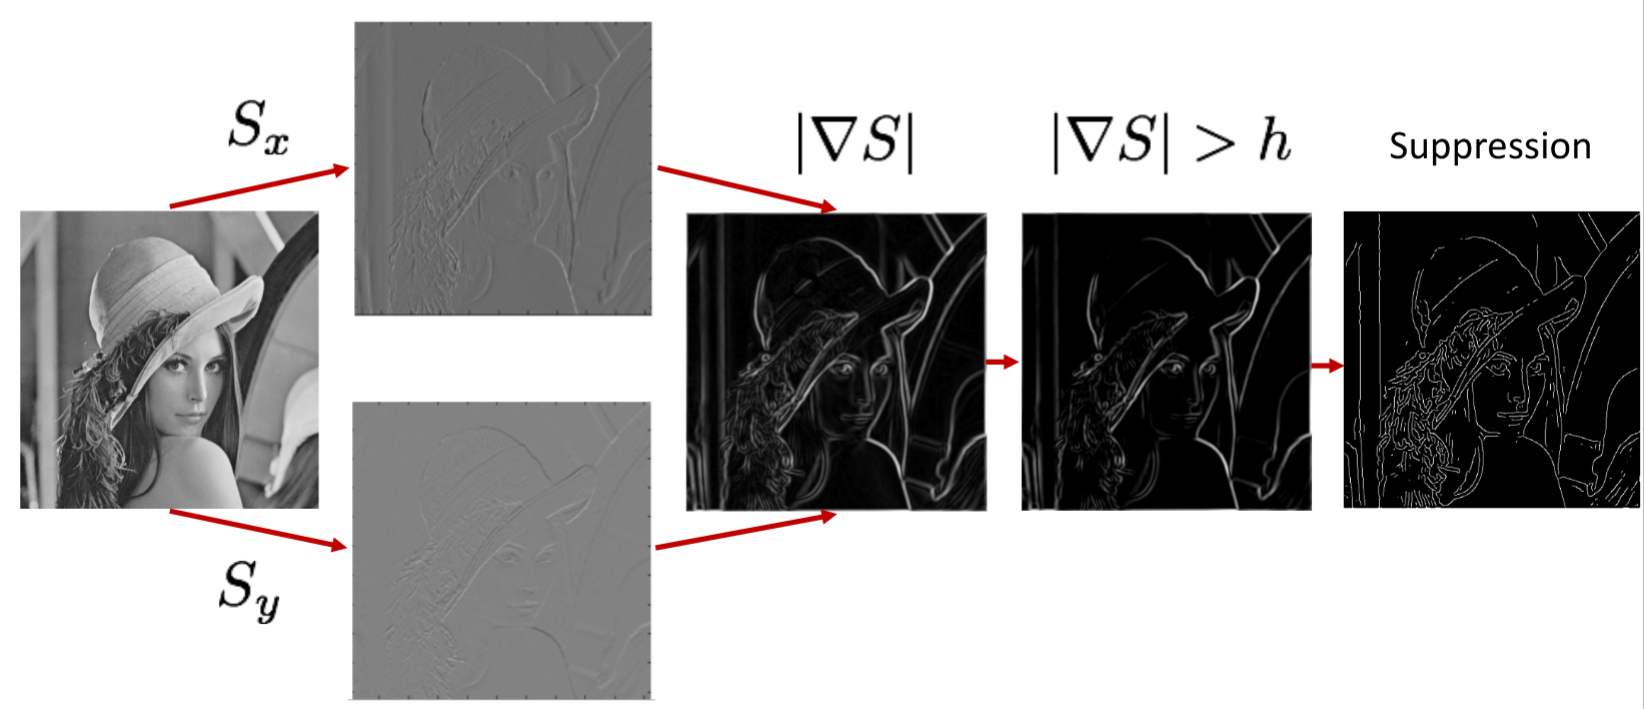
\includegraphics[scale=.32]{application.PNG}
    \caption{Classic example of 2D edge detection}
    \label{edge_app}
\end{figure}

\textbf{Corner}\\
A corner in an image is defined as an intersection of two or more edges, or as defined by Moravec \cite{Moravec}, a point where there is a large intensity variation in every direction. As shown in Fig. \ref{corner}, for a window which is centered at a pixel in a region of uniform intensity (a ``flat" region), its adjacent windows in all directions will be identical. For a window centered at a pixel on an edge, the adjacent windows will look the same except for the ones in the direction perpendicular to the edge. For a window centered at a pixel on a corner, the adjacent windows in any direction will look different.
\begin{figure}
	\centering
	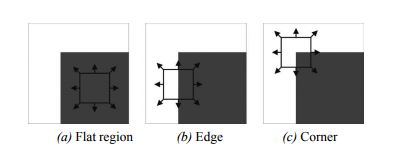
\includegraphics{corner.JPG}
    \caption{a) ``Flat'' region: no change in all directions. b) ``Edge'': no change along the edge direction. c) ``Corner'': significant changes in all directions. \cite{SNS}}
    \label{corner}
\end{figure}

Moravec's method identifies a corner where the Sum of Squared Difference (SSD) is at its local maxima. The SSD between image patch centered on pixel coordinate $(u,v)$ and the image patch shifted by $(x,y)$ is given by:
\begin{equation}
SSD(x,y) = \sum_u \sum_v ((I(u,v)-I(u+x,v+y))^2
\end{equation}
where $I$ denotes the intensity of a grayscale image. \\

\textbf{Desired properties of corner detectors}\\
The most important desired properties of corner detectors are repeatability and distinctiveness. Having detectors with ``repeatability'' means that the same features taken at the same scene under different viewpoint and illumination conditions can be found in multiple images, which requires the features to be invariant to geometric and photometric transformations. Having detectors with ``distinctiveness" means the information carried by the patch surrounding the keypoints are highly distinctive, therefore a reliable correspondence can be established, and feature points can be distinguished and matched. Good repeatability and distinctiveness are both desirable for point matching and application such as panorama stitching and 3D reconstruction.

\textbf{Harris corner detector}\\
Instead of the shifting windows, the Harris corner detector \cite{Harris} uses partial derivatives of the SSD which improves upon Moravec's corner detector.

Harris and Stephens first approximated $I(u+x,v+y)$ with a first-order Taylor expansion; the SSD can be expressed as follows:
\begin{equation}
SSD(x,y) \approx \sum_u \sum_v (I_x(u,v)x+I_y(u,v)y)^2
\label{SSD1}
\end{equation}
where $I_x$ and $I_y$ are the partial derivatives in the $x, y$ direction respectively. The quadratic form in Eq. \ref{SSD1} can be written in a matrix form:
\begin{equation}
SSD(x,y) \approx
\begin{bmatrix}
x & y\\
\end{bmatrix}
M
\begin{bmatrix}
x \\y
\end{bmatrix}
\end{equation}
where $M$ is the second moment matrix

\begin{equation}
M =
\begin{bmatrix}
\sum \sum I_x^2 & \sum \sum I_x I_y \\
\sum \sum I_x I_y & \sum \sum I_y^2 \\
\end{bmatrix}
\end{equation}

Because $M$ is symmetric, $M$ can be decomposed as:
\begin{equation}
M =
R^{-1}
\begin{bmatrix}
\lambda_1 & 0\\
0 & \lambda_2\\
\end{bmatrix}
R
\end{equation}
where $\lambda_1$ and $\lambda_2$ are the eigenvalues of $M$.
\begin{figure}
	\centering
	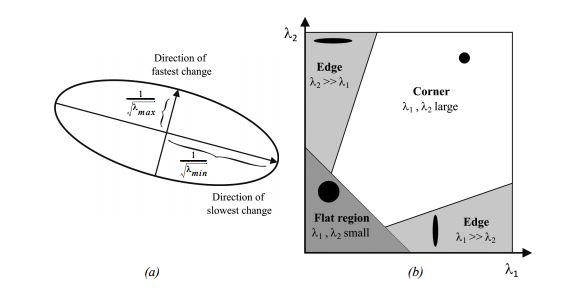
\includegraphics{harris.JPG}
    \caption{a) Visualization of direction of the fastest and slowest change of intensity built from matrix $M$. b) Harris and Stephens' classification of corners and edges \cite{SNS}}
    \label{harris}
\end{figure}

As shown in Fig. \ref{harris}, if both $\lambda_1$ and $\lambda_2$ are small, change in intensity in all direction is small, and therefore a flat region can be identified; if both $\lambda_1$ and $\lambda_2$ are large, indicating big SSD in all direction, then a corner is detected; if one eigenvalue is significantly higher than the other, the SSD is dominant in one direction, which indicates an edge. In order to reduce the complexity of the computation (i.e., avoiding calculation of eigenvalues), Harris and Stephens introduced the ``cornerness function,'' $C$, so that only the determinant and the trace of matrix $M$ need to be computed.
\begin{equation}
C = \lambda_1 \lambda_2 - \kappa(\lambda_1+\lambda_2)^2 = det(M) - \kappa\cdot trace^2(M)
\end{equation}
Here $\kappa$ is an empirically determined tunable sensitivity parameter, usually in the range of 0.04--0.15. Harris corner detector's last step is then to extract local maxima of the cornerness function using nonmaxima suppression (an algorithm to allow preserving only local maxima above some set threshold). \\

Harris corner detector is invariant to 2D rotations, as the eigenvalues of the second moment matrix $M$ don't change under pure rotation. Harris corner detector is also invariant to affine intensity changes ($I' = aI+b$), when the eigenvalues and the cornerness function are only rescaled by a constant factor, but the location of local maxima remains unchanged. However, Harris corner detector is not invariant to geometric affine changes and scale changes. Under geometric affine change, the neighborhood of the feature along $x$ and $y$ direction can be distorted and therefore varies the curvature. Under scale change, it is possible for a corner to be identified as an edge at a high scale but as a corner at a low scale.

\subsection{Descriptors}
Descriptors describe keypoints (local features) to be compared across images or used for object detection or matching. Like the detectors, it is also desirable for descriptors to be repeatable and distinct. A naive descriptor is an $n\times m$ window of pixel intensities centered at a keypoint, which can be normalized to be illumination invariant; however, it is not invariant to pose and scale, and is poorly distinctive.
\subsubsection{SIFT}
SIFT is short for Scale Invariant Feature Transform, invented in 1999 by Lowe \cite{SIFT}. SIFT not only incorporates all the properties of the scale-affine-invariant Harris, but also is extremely distinctive and robust to image noise, small illumination variations, and viewpoint changes. It is known for its high repeatability and high matching rate even in very challenging conditions, and it has lots of applications in object, gesture and face recognition, robotic perception and 3D modeling. SIFT features are essentially local distribution of image gradient around keypoints with highly informative content. The following briefly introduces the main steps of the SIFT algorithm. More details can be found in \cite{SIFT}.
\begin{enumerate}
\item Scale-space extrema detection: Keypoints are detected by searching for stable features across the scale space (a continuous function of scale). The stable keypoint locations are identified by computing the difference of Gaussian (DoG) of two nearby scale space image produced from repeatedly convolving Gaussians with the initial image, and selecting the local extrema where the sample point is the largest or smallest among its eight neighbors in the current image and nine neighbors in the scale above and below.
\item Keypoint localization: The keypoint localization step fits the nearby data for location, orientation, scale and ratio of principal curvatures around keypoints candidates, and rejects the ones that are below some contrast threshold or poorly localized along an edge.
\item Orientation assignment: This step assigns an orientation to a keypoint as the peak in the histogram of gradient orientation in the neighborhood of the keypoint. The keypoint descriptor is then represented relative to the dominant orientation assigned, which allows the descriptor to be rotation invariant. In the case when there are multiple peaks that are more than 80\% of the highest peak, multiple keypoints will be created all additional peaks, at the same location but with different assigned orientations.
\item Keypoint descriptor: The previous steps define local image regions by location, scale and orientation, and this step computes a highly distinctive and repeatable descriptor for this local image region. Each keypoint descriptor is built by stacking gradient histogram with 8 orientation bins for each $4\times 4 $ subregions of the neighboring region of the keypoints, and is therefore $4\times 4 \times 8 = 128$ in length. The length of keypoint descriptors can be changed by tuning the block size and orientation bin size; however, the 128 element vector is empirically determined to be the most robust to image variations.

\end{enumerate}
\bibliographystyle{ieeetr}
\bibliography{ref}

\subsubsection*{Contributors}
Winter 2019: [Your Names Here]
\\
Winter 2018: Peggy Wang, Molly Zhang, Michael Thompson, Pierre Lachevre, Cuthbert Sun, Quint Underwood

\end{document}
